\section{RQ2: Can Retraining Be Avoided, and What Is the Target?}
\label{sec:rq2}

An approximate unlearning method edits the reference model in place
instead of retraining it. This section asks whether an edited model
can substitute for the oracle. The question has two parts, and the
order matters. A method can only be judged against a target, so we
first establish what forgetting should aim at. We then measure how
close four methods come to that target.

Closeness is measured by the closure $\gapclosed$
(Eq.~\ref{eq:kappa}), evaluated on the removed year. A closure of
$0$ means the edited model still fits the removed year as well as
the reference, so nothing was forgotten. A closure of $1$ means the
edited model matches the counterfactual. A closure above $1$ means
it forgot more than the counterfactual ever did. A method fails in
either direction. Compliance means matching the counterfactual, so
forgetting too much is as noncompliant as forgetting too little.
All method results use the crisis-year deletion. The closure divides by the oracle's
memorization gap, and that denominator is near zero for the low- to
medium-volatility years, so readings there are not interpretable.

We test four methods. Finetune continues training on the retained
data. The hinge lowers the loss on the retained data while raising
the loss on the removed year, up to a fixed margin. SCRUB distills
the reference on the retained data and diverges from it on the
removed year~\cite{kurmanji2023scrub}. TS-Unlearn, which we
reimplement, is the only prior method built for time-series
forecasting~\cite{wang2026tsunlearn}. Hyperparameters were fixed in
advance and are listed in the released protocol. Plain gradient
ascent diverges in every cell and is excluded.

\subsection{The target of forgetting}

Two targets are conceivable for an unlearned model. The compliance
target asks it to behave like the retrained counterfactual. The
privacy target, adopted by TS-Unlearn, asks its predictions on the
removed year to become indistinguishable from noise. With $F'$ the
unlearned model and $X_f$ the removed windows,
\begin{equation}
\text{compliance: } F'(X_f) \approx F_{\text{ora}}(X_f),
\qquad
\text{privacy: } F'(X_f) \stackrel{d}{\to} \mathcal{N}(0,\Sigma).
\label{eq:compliance}
\end{equation}
Figure~\ref{fig:twodefs} compares the two targets in one picture.
We take the reference Transformer in the 2024 fold, delete the
crisis year, and apply TS-Unlearn at increasingly aggressive
settings, which produces a
family of unlearned models. Every model in the figure is placed by
two numbers. The horizontal axis is its skill on the removed year,
$\forgetic$. The vertical axis is its skill on the test year. The
reference model is the star at the upper right. It predicts both the
removed year and the test year well. The privacy target is the
dashed line at zero, where predictions of the removed year are no
better than noise. The compliance target is the diamond, the exact
counterfactual retrained without the year.

The diamond does not sit near the noise line. It sits next to the
reference. The counterfactual never trained on 2020, yet it predicts
2020 at $\forgetic = 0.51$, barely below the reference's $0.55$.
Nearly all skill on the removed year is generalization from the
retained years, not memory of the year itself. A model that predicts
the removed year like noise is therefore in a state the ground truth
never occupies.

The blue points show the price of chasing the noise target anyway.
As the method's settings grow more aggressive, the points move left,
toward the noise line. Test skill falls with them, from $0.49$ to
$0.42$, and the error bars widen about tenfold, so the models
closest to the noise target are also the least stable across seeds.
This happens in the 2024 fold, the lowest-volatility test year of
the study, where exact deletion itself moves skill by at most
$3\%$. The price of the noise target is paid even where deletion is
nearly free.
The reason is that on temporally correlated data the removed year's
patterns are the market's patterns, and a model cannot lose one
without losing the other. The correct target is the counterfactual.

The closure $\gapclosed$ measures progress along the horizontal
axis of this figure. It asks what fraction of the star-to-diamond
distance an edited model has covered. A model still at the star has
covered none of it, so its closure is $0$. A model exactly at the
diamond has covered all of it, so its closure is $1$. A model that
moves past the diamond has a closure above $1$, and a model driven
to the noise line has a closure far above $1$. Eq.~\ref{eq:kappa}
computes this fraction on the forget loss rather than on the IC
shown here, with the same two models as anchors. The privacy target
is therefore over-forgetting taken to its limit, and the next
subsection scores every cheap method on this scale.

\begin{figure}[t]
\centering
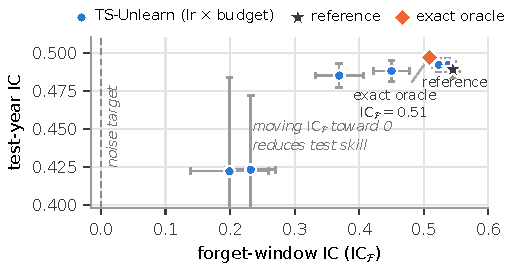
\includegraphics[width=0.92\columnwidth]{figs/fig_two_definitions}
\caption{The oracle and noise targets, compared on the Transformer
under the crisis-year deletion in the 2024 fold (\Lone). Each point
is one TS-Unlearn configuration (learning rate $\times$ budget),
averaged over ten seeds, with bars showing $\pm 1$ sd across seeds. The
dashed line marks the noise target, the diamond the exact
counterfactual, and the star the reference. The counterfactual has
higher test skill than the reference because deleting the crisis year
helps this model.}
\label{fig:twodefs}
\end{figure}

\begin{figure}[t]
\centering
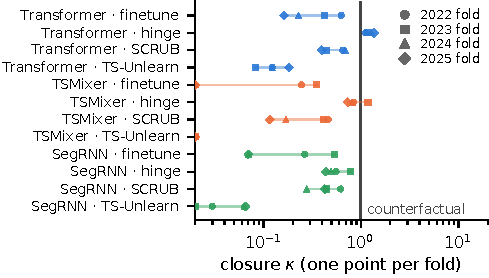
\includegraphics[width=0.92\columnwidth]{figs/fig_methods}
\caption{Closure $\gapclosed$ for each deployable
architecture-method pair on the crisis-year deletion (\Lone, 10
seeds, every method at its fixed a-priori hyperparameters), one
marker per fold, with a thin line connecting a pair's four folds. A
pair substitutes for the oracle only where its markers sit at the
counterfactual line. Values at or below zero are clipped to the
left edge of the log axis.}
\label{fig:methods}
\end{figure}

\subsection{Substitution for the oracle}

Figure~\ref{fig:methods} evaluates the four methods on the three
deployable architectures. The two non-deployable ones are omitted
from the figure. Each row is one architecture-method pair, with one
marker per fold. The test year plays no part in the closure. What
changes across folds is the training window and the position of
2020 inside it. Tightly clustered markers are a method that tracks
the oracle wherever the window sits. Scattered markers are a method
whose forgetting depends on the window it is applied to. The
vertical line at $\gapclosed = 1$ marks the counterfactual. In any
single fold, several pairs look adequate. Across all four, only
one pair stays close to the counterfactual line. The hinge on
TSMixer reaches closures of $0.74$ to $1.18$, crossing the line
from both sides and never straying from it by more than a quarter
of the gap, at no measurable cost in test skill. The hinge on the Transformer is second best; it
always overshoots, but never by more than half the gap. No other
pair stays within half the gap in every fold. For finetune, the
hinge, and SCRUB, the common failure is under-forgetting rather
than damage to the model.

TS-Unlearn fails at both of its budgets. Figure~\ref{fig:methods}
runs every method at the fixed protocol budget, and at that budget
TS-Unlearn forgets almost nothing, with
closures of $0.2$ or less on every architecture. The fixed budget
is not even harmless. In the bear-market fold, TS-Unlearn's test
skill falls $0.07$--$0.13$ IC short of the oracle and below the
reference itself, so it damages the model while forgetting almost
nothing. The sweep of
Figure~\ref{fig:twodefs} raised that budget deliberately, and there
it overshoots the counterfactual and destroys the model. A method
aimed at the noise target has no useful stopping point between the
two.

The rankings do not transfer across architectures. The same hinge
under-forgets on SegRNN, brackets the counterfactual on TSMixer,
and overshoots on the Transformer. On the non-deployable pair,
summarized in Table~\ref{tab:method_choice} and reported in full in
the released artifacts, the failures grow. The hinge
overshoots about fivefold on iTransformer, and SCRUB spans two
orders of magnitude across seeds on PatchTST, where the best-method
criterion itself degenerates: the method nearest the counterfactual
is the one that barely forgets. Nothing we measured
predicts which architecture a method will serve, and in particular
it is not the architecture with the largest memorization gap.

The fold scatter follows no rule either. Which fold lands high and
which lands low changes from pair to pair, so no fold-dependent
rule of thumb corrects a method's bias. The oracle's own gap for
the 2020 deletion varies by less than half across folds on the
deployable architectures, while the method scatter crosses from one
side of the counterfactual to the other, so the scatter comes from
the methods themselves, not from the yardstick.
Table~\ref{tab:method_choice} lists, for each architecture, the
best method under its worst fold.

The practical conclusion is that the oracle cannot be bypassed. A
closure of $1$ is defined by the oracle's fit to the removed year,
so without retraining a model owner cannot locate the target a
method is supposed to hit. The one combination that reaches the
target, the hinge on TSMixer, stops at a margin that must be set
from exactly that quantity. The figure shows that no substitute
locates the target either. Another architecture's result does not
transfer, another window position's result does not transfer, and
the memorization gap does not predict it. Validation against one's
own oracle is the only trustworthy acceptance test. It must be
repeated as the window slides, and at this scale each run costs
minutes.

\begin{table}[t]
\caption{The best method per deployable architecture, selected to
minimize the maximum $|\gapclosed-1|$ across folds. The closure range
spans the four folds. Skill cost is the worst-fold decrease in test IC
relative to the paired oracle, and the last column is wall-clock
cost relative to retraining.}
\label{tab:method_choice}
\centering
\footnotesize
\begin{tabular}{llccc}
\toprule
Architecture & Best method & Closure $\gapclosed$ & Skill cost & Cost \\
\midrule
TSMixer & hinge & $0.74$--$1.18$ & $0.004$ & $0.4\times$ \\
Transformer & hinge & $1.12$--$1.36$ & $0.011$ & $0.4\times$ \\
SegRNN & hinge & $0.44$--$0.79$ & $0.004$ & $0.2\times$ \\
\bottomrule
\end{tabular}
% Verified 2026-08-08 from the grid (worst-fold |kappa-1| criterion):
% hinge is the best on all three deployable archs; SCRUB on
% iTransformer confirmed. PatchTST's mechanical winner is TS-Unlearn
% at kappa 0.07-0.17, i.e. closest to 1 only because it barely
% forgets; 'none reliable' is the honest entry. Costs are mean method
% seconds over the era-2020 cells divided by the median oracle
% seconds of the same architecture and fold.
\end{table}
